\documentclass{standalone}
\usepackage{xcolor}
\usepackage{tikz}
\usetikzlibrary{positioning, shapes.multipart, calc, graphs, graphs.standard}
\begin{document}
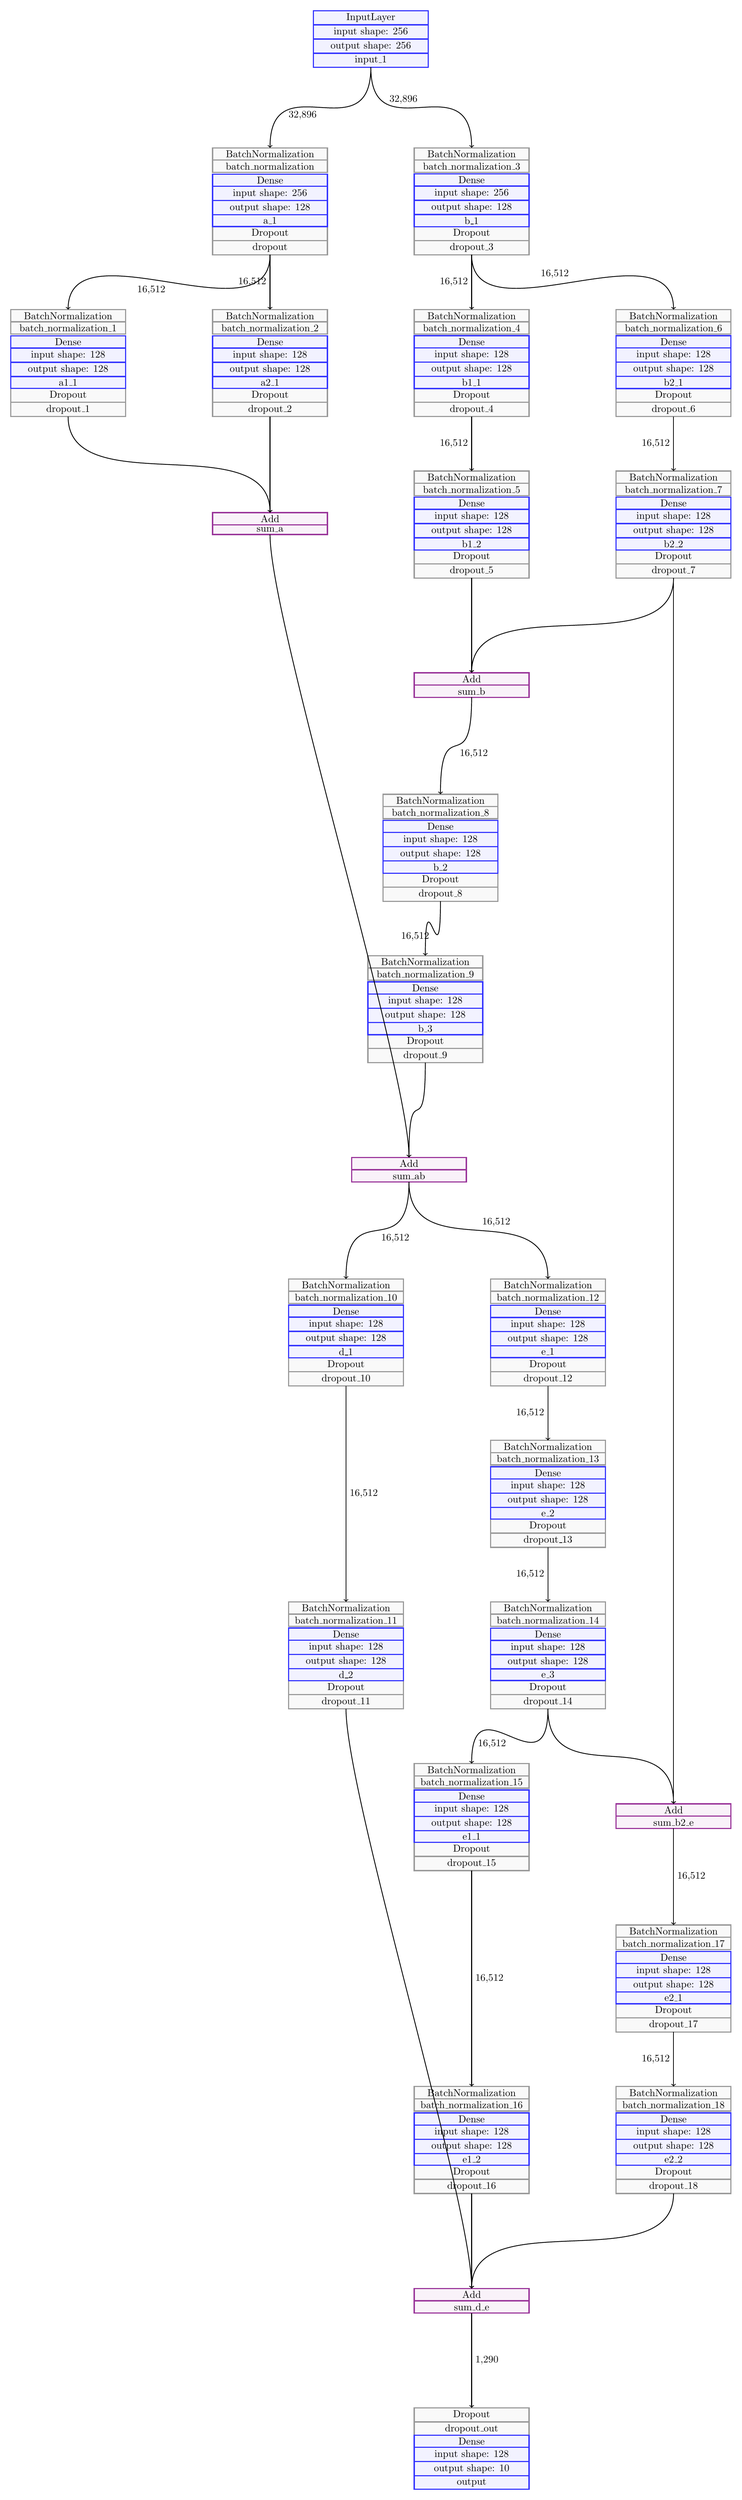
\begin{tikzpicture}[x=15.0pt, y=15.0pt, scale=2.0]
% style: major_grid
\tikzstyle{major_grid}=[black,step=20pt]
% style: minor_grid
\tikzstyle{minor_grid}=[very thin,step=10pt]
% style: defaultEdge
\tikzstyle{defaultEdge}=[thick,out=-90,in=90,out distance=1.5cm,in distance=1.5cm,looseness=1.5]
% style: defaultLabel
\tikzstyle{defaultLabel}=[auto,pos=0.5]
% style: OperationLayer_style
\tikzstyle{OperationLayer_style}=[rectangle split,rectangle split ignore empty parts,very thick,rectangle split parts=5,draw=violet!80,fill=violet!5,minimum width=4cm,outer sep=0cm,inner sep=2pt]
% style: UtilityLayer_style
\tikzstyle{UtilityLayer_style}=[rectangle split,rectangle split ignore empty parts,very thick,rectangle split parts=5,draw=gray!80,fill=gray!5,minimum width=4cm,outer sep=0cm,inner sep=2pt]
% style: TrainableLayer_style
\tikzstyle{TrainableLayer_style}=[rectangle split,rectangle split ignore empty parts,very thick,rectangle split parts=5,draw=blue!80,fill=blue!5,minimum width=4cm,outer sep=0cm,inner sep=2pt]

% node group: input_1_group
% node: input_1
\node[TrainableLayer_style] (input_1) at (10.0, 80.0)
    {
    \nodepart{one}{InputLayer}
    \nodepart{two}{input shape: 256}
    \nodepart{three}{output shape: 256}
    \nodepart{four}{input\_1}};
% end of node group: input_1_group

% node group: b_1_group
% node: batch_normalization_3
\node[UtilityLayer_style] (batch_normalization_3) at (13.33, 76.0)
    {
    \nodepart{one}{BatchNormalization}
    \nodepart{two}{batch\_normalization\_3}};
% node: dropout_3
\node[UtilityLayer_style] (dropout_3) at (13.33, 73.34)
    {
    \nodepart{one}{Dropout}
    \nodepart{two}{dropout\_3}};
% node: b_1
\node[TrainableLayer_style] (b_1) at (13.33, 74.67)
    {
    \nodepart{one}{Dense}
    \nodepart{two}{input shape: 256}
    \nodepart{three}{output shape: 128}
    \nodepart{four}{b\_1}};
% end of node group: b_1_group

% node group: a_1_group
% node: batch_normalization
\node[UtilityLayer_style] (batch_normalization) at (6.67, 76.0)
    {
    \nodepart{one}{BatchNormalization}
    \nodepart{two}{batch\_normalization}};
% node: dropout
\node[UtilityLayer_style] (dropout) at (6.67, 73.34)
    {
    \nodepart{one}{Dropout}
    \nodepart{two}{dropout}};
% node: a_1
\node[TrainableLayer_style] (a_1) at (6.67, 74.67)
    {
    \nodepart{one}{Dense}
    \nodepart{two}{input shape: 256}
    \nodepart{three}{output shape: 128}
    \nodepart{four}{a\_1}};
% end of node group: a_1_group

% node group: b1_1_group
% node: batch_normalization_4
\node[UtilityLayer_style] (batch_normalization_4) at (13.33, 70.66)
    {
    \nodepart{one}{BatchNormalization}
    \nodepart{two}{batch\_normalization\_4}};
% node: dropout_4
\node[UtilityLayer_style] (dropout_4) at (13.33, 68.0)
    {
    \nodepart{one}{Dropout}
    \nodepart{two}{dropout\_4}};
% node: b1_1
\node[TrainableLayer_style] (b1_1) at (13.33, 69.33)
    {
    \nodepart{one}{Dense}
    \nodepart{two}{input shape: 128}
    \nodepart{three}{output shape: 128}
    \nodepart{four}{b1\_1}};
% end of node group: b1_1_group

% node group: b2_1_group
% node: batch_normalization_6
\node[UtilityLayer_style] (batch_normalization_6) at (20.0, 70.66)
    {
    \nodepart{one}{BatchNormalization}
    \nodepart{two}{batch\_normalization\_6}};
% node: dropout_6
\node[UtilityLayer_style] (dropout_6) at (20.0, 68.0)
    {
    \nodepart{one}{Dropout}
    \nodepart{two}{dropout\_6}};
% node: b2_1
\node[TrainableLayer_style] (b2_1) at (20.0, 69.33)
    {
    \nodepart{one}{Dense}
    \nodepart{two}{input shape: 128}
    \nodepart{three}{output shape: 128}
    \nodepart{four}{b2\_1}};
% end of node group: b2_1_group

% node group: a1_1_group
% node: batch_normalization_1
\node[UtilityLayer_style] (batch_normalization_1) at (0.0, 70.66)
    {
    \nodepart{one}{BatchNormalization}
    \nodepart{two}{batch\_normalization\_1}};
% node: dropout_1
\node[UtilityLayer_style] (dropout_1) at (0.0, 68.0)
    {
    \nodepart{one}{Dropout}
    \nodepart{two}{dropout\_1}};
% node: a1_1
\node[TrainableLayer_style] (a1_1) at (0.0, 69.33)
    {
    \nodepart{one}{Dense}
    \nodepart{two}{input shape: 128}
    \nodepart{three}{output shape: 128}
    \nodepart{four}{a1\_1}};
% end of node group: a1_1_group

% node group: a2_1_group
% node: batch_normalization_2
\node[UtilityLayer_style] (batch_normalization_2) at (6.67, 70.66)
    {
    \nodepart{one}{BatchNormalization}
    \nodepart{two}{batch\_normalization\_2}};
% node: dropout_2
\node[UtilityLayer_style] (dropout_2) at (6.67, 68.0)
    {
    \nodepart{one}{Dropout}
    \nodepart{two}{dropout\_2}};
% node: a2_1
\node[TrainableLayer_style] (a2_1) at (6.67, 69.33)
    {
    \nodepart{one}{Dense}
    \nodepart{two}{input shape: 128}
    \nodepart{three}{output shape: 128}
    \nodepart{four}{a2\_1}};
% end of node group: a2_1_group

% node group: sum_a_group
% node: sum_a
\node[OperationLayer_style] (sum_a) at (6.67, 64.0)
    {
    \nodepart{one}{Add}
    \nodepart{two}{sum\_a}};
% end of node group: sum_a_group

% node group: b1_2_group
% node: batch_normalization_5
\node[UtilityLayer_style] (batch_normalization_5) at (13.33, 65.33)
    {
    \nodepart{one}{BatchNormalization}
    \nodepart{two}{batch\_normalization\_5}};
% node: dropout_5
\node[UtilityLayer_style] (dropout_5) at (13.33, 62.67)
    {
    \nodepart{one}{Dropout}
    \nodepart{two}{dropout\_5}};
% node: b1_2
\node[TrainableLayer_style] (b1_2) at (13.33, 64.0)
    {
    \nodepart{one}{Dense}
    \nodepart{two}{input shape: 128}
    \nodepart{three}{output shape: 128}
    \nodepart{four}{b1\_2}};
% end of node group: b1_2_group

% node group: b2_2_group
% node: batch_normalization_7
\node[UtilityLayer_style] (batch_normalization_7) at (20.0, 65.33)
    {
    \nodepart{one}{BatchNormalization}
    \nodepart{two}{batch\_normalization\_7}};
% node: dropout_7
\node[UtilityLayer_style] (dropout_7) at (20.0, 62.67)
    {
    \nodepart{one}{Dropout}
    \nodepart{two}{dropout\_7}};
% node: b2_2
\node[TrainableLayer_style] (b2_2) at (20.0, 64.0)
    {
    \nodepart{one}{Dense}
    \nodepart{two}{input shape: 128}
    \nodepart{three}{output shape: 128}
    \nodepart{four}{b2\_2}};
% end of node group: b2_2_group

% node group: sum_ab_group
% node: sum_ab
\node[OperationLayer_style] (sum_ab) at (11.26, 42.67)
    {
    \nodepart{one}{Add}
    \nodepart{two}{sum\_ab}};
% end of node group: sum_ab_group

% node group: sum_b_group
% node: sum_b
\node[OperationLayer_style] (sum_b) at (13.33, 58.67)
    {
    \nodepart{one}{Add}
    \nodepart{two}{sum\_b}};
% end of node group: sum_b_group

% node group: sum_b2_e_group
% node: sum_b2_e
\node[OperationLayer_style] (sum_b2_e) at (20.0, 21.33)
    {
    \nodepart{one}{Add}
    \nodepart{two}{sum\_b2\_e}};
% end of node group: sum_b2_e_group

% node group: e_1_group
% node: batch_normalization_12
\node[UtilityLayer_style] (batch_normalization_12) at (15.85, 38.66)
    {
    \nodepart{one}{BatchNormalization}
    \nodepart{two}{batch\_normalization\_12}};
% node: dropout_12
\node[UtilityLayer_style] (dropout_12) at (15.85, 36.0)
    {
    \nodepart{one}{Dropout}
    \nodepart{two}{dropout\_12}};
% node: e_1
\node[TrainableLayer_style] (e_1) at (15.85, 37.33)
    {
    \nodepart{one}{Dense}
    \nodepart{two}{input shape: 128}
    \nodepart{three}{output shape: 128}
    \nodepart{four}{e\_1}};
% end of node group: e_1_group

% node group: d_1_group
% node: batch_normalization_10
\node[UtilityLayer_style] (batch_normalization_10) at (9.18, 38.66)
    {
    \nodepart{one}{BatchNormalization}
    \nodepart{two}{batch\_normalization\_10}};
% node: dropout_10
\node[UtilityLayer_style] (dropout_10) at (9.18, 36.0)
    {
    \nodepart{one}{Dropout}
    \nodepart{two}{dropout\_10}};
% node: d_1
\node[TrainableLayer_style] (d_1) at (9.18, 37.33)
    {
    \nodepart{one}{Dense}
    \nodepart{two}{input shape: 128}
    \nodepart{three}{output shape: 128}
    \nodepart{four}{d\_1}};
% end of node group: d_1_group

% node group: b_2_group
% node: batch_normalization_8
\node[UtilityLayer_style] (batch_normalization_8) at (12.3, 54.66)
    {
    \nodepart{one}{BatchNormalization}
    \nodepart{two}{batch\_normalization\_8}};
% node: dropout_8
\node[UtilityLayer_style] (dropout_8) at (12.3, 52.0)
    {
    \nodepart{one}{Dropout}
    \nodepart{two}{dropout\_8}};
% node: b_2
\node[TrainableLayer_style] (b_2) at (12.3, 53.33)
    {
    \nodepart{one}{Dense}
    \nodepart{two}{input shape: 128}
    \nodepart{three}{output shape: 128}
    \nodepart{four}{b\_2}};
% end of node group: b_2_group

% node group: e2_1_group
% node: batch_normalization_17
\node[UtilityLayer_style] (batch_normalization_17) at (20.0, 17.33)
    {
    \nodepart{one}{BatchNormalization}
    \nodepart{two}{batch\_normalization\_17}};
% node: dropout_17
\node[UtilityLayer_style] (dropout_17) at (20.0, 14.67)
    {
    \nodepart{one}{Dropout}
    \nodepart{two}{dropout\_17}};
% node: e2_1
\node[TrainableLayer_style] (e2_1) at (20.0, 16.0)
    {
    \nodepart{one}{Dense}
    \nodepart{two}{input shape: 128}
    \nodepart{three}{output shape: 128}
    \nodepart{four}{e2\_1}};
% end of node group: e2_1_group

% node group: e_2_group
% node: batch_normalization_13
\node[UtilityLayer_style] (batch_normalization_13) at (15.85, 33.33)
    {
    \nodepart{one}{BatchNormalization}
    \nodepart{two}{batch\_normalization\_13}};
% node: dropout_13
\node[UtilityLayer_style] (dropout_13) at (15.85, 30.67)
    {
    \nodepart{one}{Dropout}
    \nodepart{two}{dropout\_13}};
% node: e_2
\node[TrainableLayer_style] (e_2) at (15.85, 32.0)
    {
    \nodepart{one}{Dense}
    \nodepart{two}{input shape: 128}
    \nodepart{three}{output shape: 128}
    \nodepart{four}{e\_2}};
% end of node group: e_2_group

% node group: d_2_group
% node: batch_normalization_11
\node[UtilityLayer_style] (batch_normalization_11) at (9.18, 28.0)
    {
    \nodepart{one}{BatchNormalization}
    \nodepart{two}{batch\_normalization\_11}};
% node: dropout_11
\node[UtilityLayer_style] (dropout_11) at (9.18, 25.34)
    {
    \nodepart{one}{Dropout}
    \nodepart{two}{dropout\_11}};
% node: d_2
\node[TrainableLayer_style] (d_2) at (9.18, 26.67)
    {
    \nodepart{one}{Dense}
    \nodepart{two}{input shape: 128}
    \nodepart{three}{output shape: 128}
    \nodepart{four}{d\_2}};
% end of node group: d_2_group

% node group: b_3_group
% node: batch_normalization_9
\node[UtilityLayer_style] (batch_normalization_9) at (11.8, 49.33)
    {
    \nodepart{one}{BatchNormalization}
    \nodepart{two}{batch\_normalization\_9}};
% node: dropout_9
\node[UtilityLayer_style] (dropout_9) at (11.8, 46.67)
    {
    \nodepart{one}{Dropout}
    \nodepart{two}{dropout\_9}};
% node: b_3
\node[TrainableLayer_style] (b_3) at (11.8, 48.0)
    {
    \nodepart{one}{Dense}
    \nodepart{two}{input shape: 128}
    \nodepart{three}{output shape: 128}
    \nodepart{four}{b\_3}};
% end of node group: b_3_group

% node group: e2_2_group
% node: batch_normalization_18
\node[UtilityLayer_style] (batch_normalization_18) at (20.0, 12.0)
    {
    \nodepart{one}{BatchNormalization}
    \nodepart{two}{batch\_normalization\_18}};
% node: dropout_18
\node[UtilityLayer_style] (dropout_18) at (20.0, 9.34)
    {
    \nodepart{one}{Dropout}
    \nodepart{two}{dropout\_18}};
% node: e2_2
\node[TrainableLayer_style] (e2_2) at (20.0, 10.67)
    {
    \nodepart{one}{Dense}
    \nodepart{two}{input shape: 128}
    \nodepart{three}{output shape: 128}
    \nodepart{four}{e2\_2}};
% end of node group: e2_2_group

% node group: sum_d_e_group
% node: sum_d_e
\node[OperationLayer_style] (sum_d_e) at (13.33, 5.33)
    {
    \nodepart{one}{Add}
    \nodepart{two}{sum\_d\_e}};
% end of node group: sum_d_e_group

% node group: e_3_group
% node: batch_normalization_14
\node[UtilityLayer_style] (batch_normalization_14) at (15.85, 28.0)
    {
    \nodepart{one}{BatchNormalization}
    \nodepart{two}{batch\_normalization\_14}};
% node: dropout_14
\node[UtilityLayer_style] (dropout_14) at (15.85, 25.34)
    {
    \nodepart{one}{Dropout}
    \nodepart{two}{dropout\_14}};
% node: e_3
\node[TrainableLayer_style] (e_3) at (15.85, 26.67)
    {
    \nodepart{one}{Dense}
    \nodepart{two}{input shape: 128}
    \nodepart{three}{output shape: 128}
    \nodepart{four}{e\_3}};
% end of node group: e_3_group

% node group: output_group
% node: dropout_out
\node[UtilityLayer_style] (dropout_out) at (13.33, 1.33)
    {
    \nodepart{one}{Dropout}
    \nodepart{two}{dropout\_out}};
% node: output
\node[TrainableLayer_style] (output) at (13.33, 0.0)
    {
    \nodepart{one}{Dense}
    \nodepart{two}{input shape: 128}
    \nodepart{three}{output shape: 10}
    \nodepart{four}{output}};
% end of node group: output_group

% node group: e1_1_group
% node: batch_normalization_15
\node[UtilityLayer_style] (batch_normalization_15) at (13.33, 22.66)
    {
    \nodepart{one}{BatchNormalization}
    \nodepart{two}{batch\_normalization\_15}};
% node: dropout_15
\node[UtilityLayer_style] (dropout_15) at (13.33, 20.0)
    {
    \nodepart{one}{Dropout}
    \nodepart{two}{dropout\_15}};
% node: e1_1
\node[TrainableLayer_style] (e1_1) at (13.33, 21.33)
    {
    \nodepart{one}{Dense}
    \nodepart{two}{input shape: 128}
    \nodepart{three}{output shape: 128}
    \nodepart{four}{e1\_1}};
% end of node group: e1_1_group

% node group: e1_2_group
% node: batch_normalization_16
\node[UtilityLayer_style] (batch_normalization_16) at (13.33, 12.0)
    {
    \nodepart{one}{BatchNormalization}
    \nodepart{two}{batch\_normalization\_16}};
% node: dropout_16
\node[UtilityLayer_style] (dropout_16) at (13.33, 9.34)
    {
    \nodepart{one}{Dropout}
    \nodepart{two}{dropout\_16}};
% node: e1_2
\node[TrainableLayer_style] (e1_2) at (13.33, 10.67)
    {
    \nodepart{one}{Dense}
    \nodepart{two}{input shape: 128}
    \nodepart{three}{output shape: 128}
    \nodepart{four}{e1\_2}};
% end of node group: e1_2_group

% edge from input_1 to batch_normalization_3
\draw[->, defaultEdge] (input_1) to node [defaultLabel] {32,896} (batch_normalization_3);

% edge from input_1 to batch_normalization
\draw[->, defaultEdge] (input_1) to node [defaultLabel] {32,896} (batch_normalization);

% edge from dropout_3 to batch_normalization_4
\draw[->, defaultEdge] (dropout_3) to node [defaultLabel] {16,512} (batch_normalization_4);

% edge from dropout_3 to batch_normalization_6
\draw[->, defaultEdge] (dropout_3) to node [defaultLabel] {16,512} (batch_normalization_6);

% edge from dropout to batch_normalization_1
\draw[->, defaultEdge] (dropout) to node [defaultLabel] {16,512} (batch_normalization_1);

% edge from dropout to batch_normalization_2
\draw[->, defaultEdge] (dropout) to node [defaultLabel] {16,512} (batch_normalization_2);

% edge from dropout_4 to batch_normalization_5
\draw[->, defaultEdge] (dropout_4) to node [defaultLabel] {16,512} (batch_normalization_5);

% edge from dropout_6 to batch_normalization_7
\draw[->, defaultEdge] (dropout_6) to node [defaultLabel] {16,512} (batch_normalization_7);

% edge from dropout_1 to sum_a
\draw[->, defaultEdge] (dropout_1) to node [defaultLabel] {} (sum_a);

% edge from dropout_2 to sum_a
\draw[->, defaultEdge] (dropout_2) to node [defaultLabel] {} (sum_a);

% edge from sum_a to sum_ab
\draw[->, defaultEdge] (sum_a) to node [defaultLabel] {} (sum_ab);

% edge from dropout_5 to sum_b
\draw[->, defaultEdge] (dropout_5) to node [defaultLabel] {} (sum_b);

% edge from dropout_7 to sum_b
\draw[->, defaultEdge] (dropout_7) to node [defaultLabel] {} (sum_b);

% edge from dropout_7 to sum_b2_e
\draw[->, defaultEdge] (dropout_7) to node [defaultLabel] {} (sum_b2_e);

% edge from sum_ab to batch_normalization_12
\draw[->, defaultEdge] (sum_ab) to node [defaultLabel] {16,512} (batch_normalization_12);

% edge from sum_ab to batch_normalization_10
\draw[->, defaultEdge] (sum_ab) to node [defaultLabel] {16,512} (batch_normalization_10);

% edge from sum_b to batch_normalization_8
\draw[->, defaultEdge] (sum_b) to node [defaultLabel] {16,512} (batch_normalization_8);

% edge from sum_b2_e to batch_normalization_17
\draw[->, defaultEdge] (sum_b2_e) to node [defaultLabel] {16,512} (batch_normalization_17);

% edge from dropout_12 to batch_normalization_13
\draw[->, defaultEdge] (dropout_12) to node [defaultLabel] {16,512} (batch_normalization_13);

% edge from dropout_10 to batch_normalization_11
\draw[->, defaultEdge] (dropout_10) to node [defaultLabel] {16,512} (batch_normalization_11);

% edge from dropout_8 to batch_normalization_9
\draw[->, defaultEdge] (dropout_8) to node [defaultLabel] {16,512} (batch_normalization_9);

% edge from dropout_17 to batch_normalization_18
\draw[->, defaultEdge] (dropout_17) to node [defaultLabel] {16,512} (batch_normalization_18);

% edge from dropout_13 to batch_normalization_14
\draw[->, defaultEdge] (dropout_13) to node [defaultLabel] {16,512} (batch_normalization_14);

% edge from dropout_11 to sum_d_e
\draw[->, defaultEdge] (dropout_11) to node [defaultLabel] {} (sum_d_e);

% edge from dropout_9 to sum_ab
\draw[->, defaultEdge] (dropout_9) to node [defaultLabel] {} (sum_ab);

% edge from dropout_18 to sum_d_e
\draw[->, defaultEdge] (dropout_18) to node [defaultLabel] {} (sum_d_e);

% edge from sum_d_e to dropout_out
\draw[->, defaultEdge] (sum_d_e) to node [defaultLabel] {1,290} (dropout_out);

% edge from dropout_14 to sum_b2_e
\draw[->, defaultEdge] (dropout_14) to node [defaultLabel] {} (sum_b2_e);

% edge from dropout_14 to batch_normalization_15
\draw[->, defaultEdge] (dropout_14) to node [defaultLabel] {16,512} (batch_normalization_15);

% edge from dropout_15 to batch_normalization_16
\draw[->, defaultEdge] (dropout_15) to node [defaultLabel] {16,512} (batch_normalization_16);

% edge from dropout_16 to sum_d_e
\draw[->, defaultEdge] (dropout_16) to node [defaultLabel] {} (sum_d_e);

\end{tikzpicture}\end{document}